%%% Template originaly created by Karol Kozioł (mail@karol-koziol.net) and modified for ShareLaTeX use

\documentclass[a4paper,11pt]{article}

\usepackage[T1]{fontenc}
\usepackage[utf8]{inputenc}
\usepackage{graphicx}
\usepackage{xcolor}
\usepackage[]{authblk}

\renewcommand\familydefault{\sfdefault}
\usepackage{tgheros}
\usepackage[defaultmono]{droidmono}

\usepackage{amsmath,amssymb,amsthm,textcomp}
\usepackage{enumerate}
\usepackage{multicol}
\usepackage{tikz}

\usepackage{geometry}
%\geometry{total={210mm,297mm},
%left=25mm,right=25mm,%
%bindingoffset=0mm, top=20mm,bottom=20mm}


\linespread{1.2}

\newcommand{\linia}{\rule{\linewidth}{0.5pt}}

% custom theorems if needed
\newtheoremstyle{mytheor}
    {1ex}{1ex}{\normalfont}{0pt}{\scshape}{.}{1ex}
    {{\thmname{#1 }}{\thmnumber{#2}}{\thmnote{ (#3)}}}

%\theoremstyle{mytheor}
%\newtheorem{defi}{Definition}

% my own titles
\makeatletter
\renewcommand{\maketitle}{
\begin{center}
\vspace{2ex}
{\LARGE \textsc{\@title}}
\vspace{1ex}
\\
\linia\\
\@author \hfill \@date
\vspace{4ex}
\end{center}
}
\makeatother
%%%

% custom footers and headers
\usepackage{fancyhdr}
\pagestyle{fancy}
\lhead{}
\chead{}
\rhead{}
\lfoot{Assignment \textnumero{} 1}
\cfoot{}
\rfoot{Page \thepage}
\renewcommand{\headrulewidth}{0pt}
\renewcommand{\footrulewidth}{0pt}
%

% code listing settings
\usepackage{listings}
\lstset{
    language=Python,
    basicstyle=\ttfamily\small,
    aboveskip={1.0\baselineskip},
    belowskip={1.0\baselineskip},
    columns=fixed,
    extendedchars=true,
    breaklines=true,
    tabsize=4,
    prebreak=\raisebox{0ex}[0ex][0ex]{\ensuremath{\hookleftarrow}},
    frame=lines,
    showtabs=false,
    showspaces=false,
    showstringspaces=false,
    keywordstyle=\color[rgb]{0.627,0.126,0.941},
    commentstyle=\color[rgb]{0.133,0.545,0.133},
    stringstyle=\color[rgb]{01,0,0},
    numbers=left,
    numberstyle=\small,
    stepnumber=1,
    numbersep=10pt,
    captionpos=t,
    escapeinside={\%*}{*)}
}

%%%----------%%%----------%%%----------%%%----------%%%

\begin{document}

\title{Project 1: Probability Distributions and Bayesian Networks}

\author{Avinash Kommineni} 
\affil{50248877  \\ akommineni@buffalo.edu}

%\date{\today}

\maketitle

\section*{Problem 1.1}

The excel file is read and loaded into the workspace by the \textit{read\_excel} query of \textit{pandas} library as a dataframe. By selecting only the necessary columnsand omitting the others, it is easier to handle the required data. The mean($\mu$), variance($\sigma^2$) and standard deviation($\sigma$) can be calculated either from pandas inbuilt functions or numpy inbulit functions. But there is a slight difference between these two in case of variance and standard-deviation. The difference being, the \textit{df.var()} considers the number of elements as {\textit{N-1} where N is the total number of rows (49 in this case). The numpy way of calculating is called \textit{Unbiased Estimator}.
So for the above purposes, the libraries numpy and pandas are used (imported).

\begin{lstlisting}[label={list:first},caption= Calculating Mean Variance Standard deviation.]
import numpy as np
import pandas as pd

df = pd.read_excel('DataSet/university data.xlsx')
FORMAT = ['CS Score (USNews)', 'Research Overhead %', 'Admin Base Pay$', 'Tuition(out-state)$']
df = df[FORMAT]
print('UBitName = akommine')
print('personNumber = 50248877')

print('\nMeans')
mu = np.mean(df)
for i in range(mu.size):
print('mu{} {:.3f}'.format(i+1,mu[i]))

print('\nVariance')
var = df.var()
for i in range(var.size):
print('var{} {:.3f}'.format(i+1,var[i]))

print('\nVariance using Unbiased Estimator')
var2 = np.var(df)
for i in range(var2.size):
print('var{} {:.3f}'.format(i+1,var2[i]))

print('\nStandard Deviation')
std = df.std()
for i in range(std.size):
print('sigma{} {:.3f}'.format(i+1,std[i]))

print('\nStandard Deviation using Unbiased Estimator')
std2 = np.std(df)
for i in range(std2.size):
print('sigma{} {:.3f}'.format(i+1,std2[i]))
\end{lstlisting}

\section*{Problem 1.2}

All the data from dataframe is stored as array for easy access of just the values and not the labels, and also for further future purposes. The \textit{covarianceMat} and the \textit{correlationMat} are calculated from \textit{numpy}'s in-built functions \textit{np.cov} and \textit{np.corrcoef}.

\begin{lstlisting}[label={list:second},caption=Calculating covarianceMat and correlationMat matrices.]
Y = np.vstack((df['CS Score (USNews)'], df['Research Overhead %'], df['Admin Base Pay$'], df['Tuition(out-state)$']))
Y = np.delete(Y,-1,1)
covarianceMat = np.cov(Y)
np.set_printoptions(formatter={'float': lambda x: "{:0.3f}".format(x)})
print('\nCovarianceMat:\n{}'.format(np.round(covarianceMat,decimals=3)))
correlationMat = np.corrcoef(Y)
print('\ncorrelationMat:\n{}'.format(correlationMat))
\end{lstlisting}

\section*{Problem 1.3}

The \textit{logLikelihood} of the data is calculated by the formula

\[ L(\mu,\sigma^2:x_1,x_2,...,x_n) = -\frac{n}{2}\ln(2\pi\sigma^2) -\frac{n}{2\sigma^2}\sum_{i=1}^{n}(x_i - \mu)^2 \]
The equation has been implemented in a effecient way by the use of broadcasting.

\begin{lstlisting}[label={list:third},caption=Calculating logLikelihood value.]
loglike =  -(df.count()[0]/2)*np.log(2*np.pi*var2) - (0.5/var2)*np.sum((Y-mu[:,np.newaxis])**2,axis=1)
totalLog = np.sum(loglike)
print('\nlogLikelihood is: {}\n'.format(totalLog))
\end{lstlisting}

\section*{Problem 1.4}

The \textit{logLikelihood} of the multivariate gaussian distribution is calculated using the inbuilt function of multivariate\_normal from scipy library.

\begin{lstlisting}[label={list:fourth},caption=Calculating logLikelihood for multivariate gaussian.]
from scipy.stats import multivariate_normal

multivariate_normalvar = multivariate_normal.logpdf(Y.T, mu, cov = covarianceMat,allow_singular = True)
multivariate_normalvar = sum(multivariate_normalvar)
print('logLikelihood for multivariate gaussian is: {}\n'.format(multivariate_normalvar))
\end{lstlisting}


\section*{Code Output}

\begin{lstlisting}[label={list:fifth},caption=Code output.]
UBitName = akommine
personNumber = 50248877

Means
mu1 3.214
mu2 53.386
mu3 469178.816
mu4 29711.959

Variance
var1 0.457
var2 12.850
var3 14189720820.903
var4 31367695.790

Variance using Unbiased Estimator
var1 0.448
var2 12.588
var3 13900134681.701
var4 30727538.733

Standard Deviation
sigma1 0.676
sigma2 3.585
sigma3 119120.615
sigma4 5600.687

Standard Deviation using Unbiased Estimator
sigma1 0.669
sigma2 3.548
sigma3 117898.832
sigma4 5543.243

CovarianceMat:
[[0.457 1.106 3879.782 1058.480]
[1.106 12.850 70279.376 2805.789]
[3879.782 70279.376 14189720820.903 -163685641.258]
[1058.480 2805.789 -163685641.258 31367695.790]]

correlationMat:
[[1.000 0.456 0.048 0.279]
[0.456 1.000 0.165 0.140]
[0.048 0.165 1.000 -0.245]
[0.279 0.140 -0.245 1.000]]

logLikelihood is: -1315.098792560739

logLikelihood for multivariate gaussian is: -1262.32720006137
\end{lstlisting}

\section*{Results}

To better understand the correlation matrix, the following plot is drawn to portray the correlation between each of the four variables...

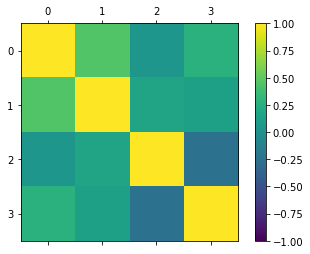
\includegraphics{plot}

The follwing are plots for each pairs of variables and a linear fit to the data.\\
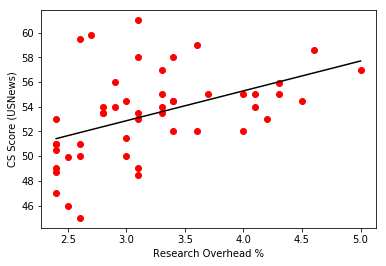
\includegraphics{0,1}\\
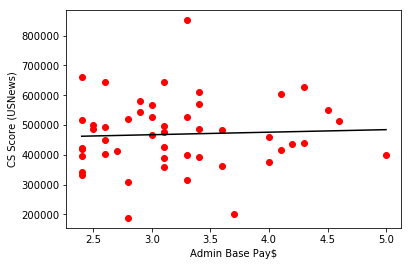
\includegraphics{0,2}\\
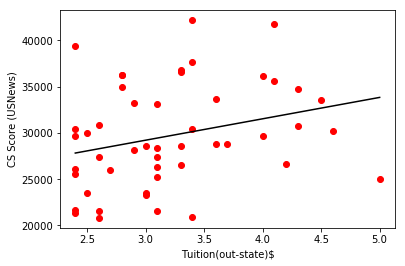
\includegraphics{0,3}\\
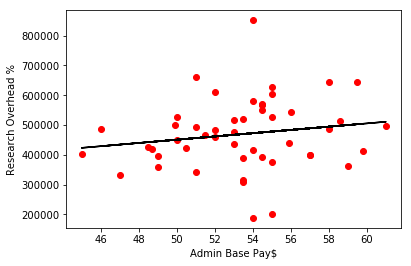
\includegraphics{1,2}\\
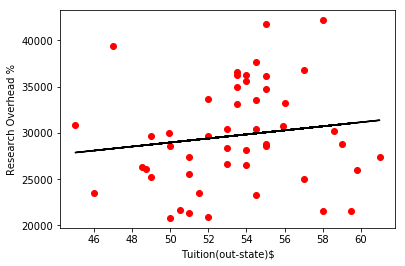
\includegraphics{1,3}\\
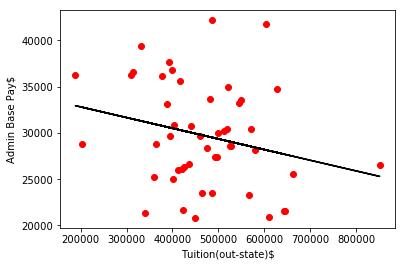
\includegraphics{2,3}


\end{document}
